\section{Problem Definition}
\subsection{Graph Problems}
\begin{frame}{The Problem Presented as Graphs}
\framesubtitle{How?}

\only<1,4>{
	\begin{itemize}
		\item Nodes are devices.
		\item Edges indicate which devices a device is in range of.
		\only<4>{
		\item Weights indicate the chance of a transmission being received.
		}
	\end{itemize}
}

\only<2>{
\begin{figure}
\centering
\begin{tikzpicture}  [
        node distance = 1 cm, 
        vertex/.style = {circle, draw, fill=blue!10}, 
        label/.style={fill=white},
        <->
    ]

    \node[draw=none](0){};
    \node[vertex, left  = 2cm of 0]   (1) {$v_1$};
    \node[vertex, above =     of 0]   (2) {$v_2$};
    \node[vertex, right = 2cm of 0]   (3) {$v_3$};
    \node[vertex, below =     of 0]   (4) {$v_4$};
    
    \draw (1) -- (2);
    \draw (1) -- (3);
    \draw (1) -- (4);
    \draw (2) -- (3);
    \draw (2) -- (4);
    \draw (3) -- (4);

\end{tikzpicture}
\end{figure}
Completely Connected Reliable Communication (CCRC).
}
\only<3>{
\begin{figure}
\centering
\begin{tikzpicture}  [
        node distance = 1 cm, 
        vertex/.style = {circle, draw, fill=blue!10}, 
        label/.style={fill=white},
        <->
    ]

    \node[draw=none](0){};
    \node[vertex, left  = 2cm of 0]   (1) {$v_1$};
    \node[vertex, above =     of 0]   (2) {$v_2$};
    \node[vertex, right = 2cm of 0]   (3) {$v_3$};
    \node[vertex, below =     of 0]   (4) {$v_4$};
    
    \draw (1) -- (2);
    \draw (1) -- (4);
    \draw (2) -- (3);
    \draw (2) -- (4);
    \draw (3) -- (4);

\end{tikzpicture}
\end{figure}
Strongly Connected Reliable Communication (SCRC).
}
\only<6>{
\begin{figure}
\centering
\begin{tikzpicture} [
        node distance = 1 cm, 
        vertex/.style = {circle, draw, fill=blue!10}, 
        edge/.style = {draw, -stealth, shorten >= 1pt},
        label/.style={fill=white}
    ]

    \node[draw=none](0){};
    \node[vertex, left =  2cm of 0]   (1) {$v_1$};
    \node[vertex, above=      of 0]   (2) {$v_2$};
    \node[vertex, right=  2cm of 0]   (3) {$v_3$};
    \node[vertex, below=      of 0]   (4) {$v_4$};
    
    \path[edge] (1) edge[bend left=15] node [label] {0.7} (2) edge[bend left=15] node [label] {0.5} (4);
    \path[edge] (2) edge[bend left=15] node [label] {0.8} (1) edge[bend left=15] node [label] {0.7} (3);
    \path[edge] (3) edge[bend left=15] node [label] {0.9} (2) edge[bend left=15] node [label] {0.8} (4);
    \path[edge] (4) edge[bend left=15] node [label] {0.4} (1) edge[bend left=15] node [label] {0.8} (3);
    
\end{tikzpicture}
\end{figure}
Strongly Connected Unreliable Communication (SCUC).
}

\only<5>{
\begin{figure}
\centering
\begin{tikzpicture} [
        node distance = 1 cm, 
        vertex/.style = {circle, draw, fill=blue!10}, 
        edge/.style = {draw, -stealth, shorten >= 1pt},
        label/.style={fill=white}
    ]

    \node[draw=none](0){};
    \node[vertex, left =  3cm of 0]   (1) {$v_1$};
    \node[vertex, above=  2cm of 0]   (2) {$v_2$};
    \node[vertex, right=  3cm of 0]   (3) {$v_3$};
    \node[vertex, below=  2cm of 0]   (4) {$v_4$};
    
    \path[edge] (1) edge[bend left=15] node [label] {0.7} (2) edge[bend left=15] node [label] {0.5} (4);
    \path[edge] (1) edge[bend left=15] node [label] {0.7} (2) edge[bend left=15] node [label] {0.3} (3);
    \path[edge] (3) edge[bend left=15] node [label] {0.7} (2) edge[bend left=15] node [label] {0.3} (1);
    \path[edge] (2) edge[bend left=15] node [label] {0.7} (1) edge[bend left=15] node [label] {0.5} (4);
    \path[edge] (4) edge[bend left=15] node [label] {0.7} (1) edge[bend left=15] node [label] {0.5} (2);
    \path[edge] (2) edge[bend left=15] node [label] {0.8} (1) edge[bend left=15] node [label] {0.7} (3);
    \path[edge] (3) edge[bend left=15] node [label] {0.9} (2) edge[bend left=15] node [label] {0.8} (4);
    \path[edge] (4) edge[bend left=15] node [label] {0.4} (1) edge[bend left=15] node [label] {0.8} (3);
    
\end{tikzpicture}
\end{figure}
Completely Connected Unreliable Communication (CCUC).
}
\end{frame}

\begin{frame}{Time Division Multiple Access(TDMA)}
\subsection{TDMA Problem}
\begin{itemize}
	\item One frequency.
	\item Using the frequency in turns.
	\item Frame and time-slots.
\end{itemize}
\vspace{-15pt}
\begin{figure}
\centering
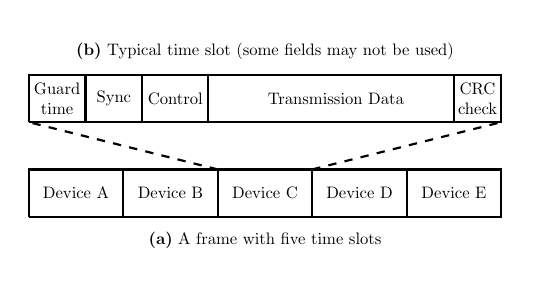
\begin{tikzpicture}[thick,scale=0.6, every node/.style={scale=0.6}]
    \path[draw] (-5,0) -- (-5,1) -- (5,1) -- (5,0) -- (-5,0)
                (-3,1) -- (-3,0)
                (-1,1) -- (-1,0)
                (1,1) -- (1,0)
                (3,1) -- (3,0);
                
    \node at (-4,0.5) {Device A};
    \node at (-2,0.5) {Device B};
    \node at (0,0.5) {Device C};
    \node at (2,0.5) {Device D};
    \node at (4,0.5) {Device E};
    
    \path[draw, dashed] (-1,1) -- (-5,2)
                        (1,1) -- (5,2);
    
    \path[draw] (-5,2) -- (-5,3) -- (5,3) -- (5,2) -- (-5,2)
                (-3.8,2) -- (-3.8,3)
                (-2.6,2) -- (-2.6,3)
                (-1.2,2) -- (-1.2,3)
                (4,2) -- (4,3);
    
    \node[text width=1cm, align=center] at (-4.4,2.5) {Guard\\time};
    \node at (-3.2,2.5) {Sync};
    \node at (-1.9,2.5) {Control};
    \node at (1.5,2.5) {Transmission Data};
    \node[text width=1cm, align=center] at (4.5,2.5) {CRC\\check};
    
    \path (-5,4) -- node{\textbf{(b)} Typical time slot (some fields may not be used)} (5,3);
    
    \path (5,-1) -- node{\textbf{(a)} A frame with five time slots} (-5,0);
\end{tikzpicture}
\end{figure}
\vspace{-15pt}
For our project:
	\begin{itemize}
		\item Devices should be able to join.
		\item The number of devices are not known in advance.
	\end{itemize}
\end{frame}

\begin{frame}{Design of CCRC}

\begin{itemize}
	\item The TDMA solution for CCRC.
	\item Joining devices wait for Empty-Slot and then connects to the network.
\end{itemize}
\begin{figure}
\centering
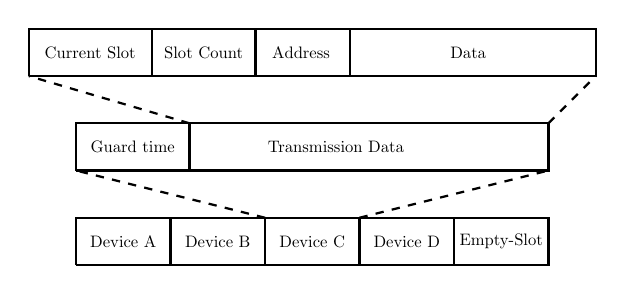
\begin{tikzpicture}[thick,scale=0.6, every node/.style={scale=0.6}]
    \path[draw] (-5,0) -- (-5,1) -- (5,1) -- (5,0) -- (-5,0)
                (-3,1) -- (-3,0)
                (-1,1) -- (-1,0)
                (1,1) -- (1,0)
                (3,1) -- (3,0);
                
    \node at (-4,0.5) {Device A};
    \node at (-2,0.5) {Device B};
    \node at (0,0.5) {Device C};
    \node at (2,0.5) {Device D};
    \node at (4,0.5) {Empty-Slot};
    
    \path[draw, dashed] (-1,1) -- (-5,2)
                        (1,1) -- (5,2);
    
    \path[draw] (-5,2) -- (-5,3) -- (5,3) -- (5,2) -- (-5,2)
                (-2.6,2) -- (-2.6,3);

    \node at (-3.8,2.5) {Guard time};
    \node at (0.5,2.5) {Transmission Data};

    \path[draw, dashed] (-2.6,3) -- (-6,4)
                        (5,3) -- (6,4);

    \path[draw] (-6,4) -- (-6,5) -- (6,5) -- (6,4) -- (-6,4)
    			(-3.4,4) -- (-3.4,5)
    			(-1.2,4) -- (-1.2,5)
    			(0.8,4) -- (0.8,5);

    \node at (-4.7,4.5) {Current Slot};
    \node at (-2.3,4.5) {Slot Count};
    \node[text width=1cm, align=center] at (-0.35,4.5) {Address};
    \node[text width=1cm, align=center] at (3.3,4.5) {Data};
    
\end{tikzpicture}
\end{figure}
\begin{itemize}
\item Presentation of CCRC in UPPAAL.
\end{itemize}
\end{frame}
